%%\documentclass[handout]{beamer}
%\documentclass[aspectratio=169,13pt]{beamer}
%\newcommand{\dee}{\partial}

\newcommand{\bmat}[1]{\begin{bmatrix} \B{#1}_{11} & \B{#1}_{12} \\ \B{#1}_{21} & \B{#1}_{22}\end{bmatrix}}
\newcommand{\blmat}[1]{\begin{bmatrix} \B{#1}_{11} &  \\ \B{#1}_{21} & \B{#1}_{22}\end{bmatrix}}
\newcommand{\brmat}[1]{\begin{bmatrix} \B{#1}_{11} & \B{#1}_{12} \\ & \B{#1}_{22}\end{bmatrix}}
\newcommand{\bomat}[1]{\begin{bmatrix} {#1}_{11} & \B{#1}_{12} \\ \B{#1}_{21} & \B{\uppercase{#1}}_{22}\end{bmatrix}}
\newcommand{\blomat}[1]{\begin{bmatrix} {#1}_{11} & \\ \B{#1}_{21} & \B{\uppercase{#1}}_{22}\end{bmatrix}}
\newcommand{\bromat}[1]{\begin{bmatrix} {#1}_{11} & \B{#1}_{12} \\  & \B{\uppercase{#1}}_{22}\end{bmatrix}}

\DeclareMathOperator{\vcop}{vec}
\newcommand{\vc}[1]{\vcop\left(#1\right)}
\newcommand{\prm}{\mu}

\newcommand{\fl}{fl}
\newcommand{\asmcond}[1]{\smallskip{\it #1}\smallskip}
\newcommand{\amdcond}[1]{\smallskip{\it #1}\smallskip}
\newcommand{\algcond}[1]{\smallskip{\it #1}\smallskip}
\newcommand{\atsmcond}[1]{{\it #1}}
\newcommand{\atmdcond}[1]{{\it #1}}
\newcommand{\atlgcond}[1]{{\it #1}}
\newcommand{\afillnum}[1]{{\underline{ \ #1\ \ }}}

\mode<presentation>
{
  \usetheme{Malmoe}
}

\usepackage[english]{babel}
%
%\usepackage[latin1]{inputenc}
%
%\usepackage{times}
%\usepackage[T1]{fontenc}
% Or whatever. Note that the encoding and the font should match. If T1
% does not look nice, try deleting the line with the fontenc.

\usepackage{inconsolata}
\usepackage{listings}
\usepackage{bm}
\usefonttheme[onlymath]{serif}
\renewcommand\familydefault{\sfdefault}
\usepackage[sfdefault]{ClearSans} %% option 'sfdefault' activates Clear Sans as the default text font
%\usefonttheme{professionalfonts}

\usepackage{latexsym}
\usepackage{amsmath}
\usepackage{amssymb}
\usepackage{amsfonts}
\usepackage{graphics}
\usepackage{multicol}

\definecolor{darkred}{rgb}{0.8,0.2,0.2}
\newcommand{\coloremph}[1]{\textcolor{darkred}{\emph{#1}}}        % colored italics
\newcommand{\reshape}[2]{o_{#1}(#2)}        % colored italics
\newcommand{\ket}[1]{\lvert #1 \rangle}
\newcommand{\bra}[1]{\langle #1 \vert}
\newcommand{\transp}[2]{{#2}^{\langle  {#1} \rangle }}        % colored italics

% Miscellaneous special math symbols

% Big-oh notation - either Latex's calligraphic O or uppercase math italic O
\newcommand{\BIGOH}{\mathcal{O}}                              % big oh
%\newcommand{\BIGOH}{O}                                       % big oh
\newcommand{\BIGTHETA}{\Theta}                                % big theta

\newcommand{\sfrac}[2]{{#1}/{#2}}

% Various versions of the fraction one-half
% solidus 1/2 for superscripts:
\newcommand{\SHALF}{1/2}                                      % one-half power
% small 1/2 set case in displayed equations:
\newcommand{\HALF}{\mbox{\small $\frac{1}{2}$}}               % small one-half
\newcommand{\THRD}{\mbox{\scriptsize $\frac{1}{3}$}}          % small one-third
\newcommand{\TWOTH}{\mbox{\scriptsize $\frac{2}{3}$}}         % small two-thirds

% Machine epsilon - note that placement of subscript may need adjustment.
%\newcommand{\emach}{\epsilon_{\textrm{\scriptsize mach}}} % machine prec.
\newcommand{\emach}{\epsilon}

\newcommand{\lsapprox}{\cong}                             % least squares approx

% Real numbers - Prefer \mathbb{R} but it requires amsfonts.
%                Latex's calligraphic R will do if amsfonts are unavailable.
%                DO NOT use \Re, which gives old German fraktur R.
\newcommand{\Real}{\mathbb{R}}                                 % real numbers
\newcommand{\Cplx}{\mathbb{C}}                                 % complex numbers
\newcommand{\Poly}{\mathbb{P}}                                 % polynomials
\newcommand{\Float}{\mathbb{F}}                                % fl pt system
% Bold math fonts for vectors and matrices
\renewcommand{\Vec}[1]{\ensuremath{\bm{#1}}}                   % vector
\newcommand{\Mat}[1]{\ensuremath{\bm{#1}}}                     % matrix
\newcommand{\Op}[1]{#1}                              % operator
\newcommand{\loc}[1]{x_{#1}}                              % operator

% Loglike functions set in regular type
\newcommand{\diag}{\mathrm{diag}}                             % diagonal matrix
\newcommand{\cond}{\mathrm{cond}}                             % condition number
\newcommand{\sign}{\mathrm{sign}}                             % sign function
\newcommand{\Span}{\text{span}}                             % span of matrix
%\newcommand{\trace}{\mathrm{trace}}                           % trace of matrix
\DeclareMathOperator*{\trace}{trace}
\newcommand{\tentrace}[3]{\trace_{#1,#2}(#3)}
\renewcommand{\Re}{\mathrm{Re}}                               % real part
\renewcommand{\Im}{\mathrm{Im}}                               % imaginary part

% Fractions appearing in matrices - allows setting them case or solidus
%\newcommand{\mf}[2]{{#1 \over #2}}        % matrix fraction - set case
\newcommand{\mf}[2]{#1/#2}               % matrix fraction - set solidus


% Keywords for algorithm statements

\newcommand{\FOR}{\textbf{for}\ }
\newcommand{\TO}{\textbf{to}\ }
\newcommand{\IF}{\textbf{if}\ }
\newcommand{\THEN}{\textbf{then}\ }
\newcommand{\ELSE}{\textbf{else}\ }
\newcommand{\WHILE}{\textbf{while}\ }
\newcommand{\DO}{\textbf{do}\ }
\newcommand{\BEGIN}{\textbf{begin}\ }
\newcommand{\END}{\textbf{end}\ }
\newcommand{\STOP}{\textbf{stop}\ }
\newcommand{\AND}{\textbf{and}\ }
\newcommand{\OR}{\textbf{or}\ }

\newcommand{\comm}{\mathrm{comm}}
\newcommand{\comp}{\mathrm{comp}}
\newcommand{\idle}{\mathrm{idle}}
\newcommand{\msg}{\mathrm{msg}}
\newcommand{\len}{\mathrm{s}}
\newcommand{\route}{\mathrm{route}}
\newcommand{\mitem}{\medskip\item}
\newcommand{\sitem}{\smallskip\item}
\DeclareMathOperator*{\argmin}{argmin}

%Gets rid of headline

\setbeamertemplate{footline}{}

\setbeamertemplate{headline}{}
\beamertemplatenavigationsymbolsempty



\definecolor{mygreen}{rgb}{0,0.2,0}
\definecolor{mygray}{rgb}{0.5,0.5,0.5}
\definecolor{mymauve}{rgb}{0.58,0,0.82}
\definecolor{mypurple}{rgb}{0.38,0,0.32}
\definecolor{myblue}{rgb}{0.2,0,0.5}
\definecolor{darkgreen}{rgb}{0.2,0.6,0.2}
\definecolor{Brown}{rgb}{0.39, 0.09, 0.0}
\definecolor{Violet}{rgb}{0.38, 0.0, 0.63}
\definecolor{myvlgray}{rgb}{0.9,0.9,1.0}
\definecolor{mylgray}{rgb}{0.85,0.85,0.9}
\definecolor{darkgreen}{rgb}{0,0.4,0}
\definecolor{brown}{rgb}{.6,.1,.1}

\newcommand{\bemph}[1]{{\color{blue} \emph{#1}}}

\usepackage{mathtools}
\newcommand{\defeq}{\coloneqq}

\newcommand{\inti}[2]{[{#1},{#2}]}
\newcommand{\BF}{\mathbf}
\newcommand{\CF}{\mathcal}
\newcommand{\B}[1]{\bm{#1}}
\newcommand{\E}[1]{\bm{#1}}
\newcommand{\dis}{\displaystyle}
\newcommand{\lt}{\left}
\newcommand{\rt}{\right}

\newcommand{\cs}{H}

\DeclareMathOperator*{\rank}{rank}
\DeclareMathOperator*{\vecn}{vec}
\DeclareMathOperator*{\vecs}{vech}

\usepackage{eso-pic}
\newcommand{\cornertext}[1]{
  \AddToShipoutPictureFG*{
    \AtPageUpperLeft{\put(0,-10){\makebox[\paperwidth][r]{#1}}}  
   }%
}
\newcommand{\cornertexttwo}[2]{
  \AddToShipoutPictureFG*{
    \AtPageUpperLeft{\put(0,-10){\makebox[\paperwidth][r]{#1}}}  
    \AtPageUpperLeft{\put(0,-20){\makebox[\paperwidth][r]{#2}}}  
   }%
}
\newcommand{\linkdemo}[2]{{\footnotesize\href{https://relate.cs.illinois.edu/course/cs450-f18/f/demos/upload/#1/#2.html}{\color{Violet}{\it\textbf{Demo:} #2}\ }}}
\newcommand{\linkinclass}[2]{{\footnotesize\href{https://relate.cs.illinois.edu/course/cs450-f18/flow/#1/start/}{\color{darkgreen}{\it\textbf{Activity:} #2}\ }}}
\newcommand{\urcornerlinkinclass}[2]{\cornertext{\linkinclass{#1}{#2}}}
\newcommand{\dblurcornerlinkinclass}[4]{\cornertexttwo{\linkinclass{#1}{#2}}{\linkinclass{#3}{#4}}}
\newcommand{\urcornerlinkdemo}[2]{\cornertext{\linkdemo{#1}{#2}}}
\newcommand{\dblurcornerlinkdemo}[4]{\cornertexttwo{\linkdemo{#1}{#2}}{\linkdemo{#3}{#4}}}
\newcommand{\urcornerlinkdemoinclass}[4]{\cornertexttwo{\linkdemo{#1}{#2}}{\linkinclass{#3}{#4}}}



% CS 554 specific:

\newcommand{\tsync}{\alpha}
\newcommand{\tword}{\beta}
\newcommand{\tflop}{\gamma}

\newcommand{\bw}{w}

\newcommand{\tpl}[2]{{\bm{#1}}}
\newcommand{\vtpl}[3]{{\bm{#1}}_#3}
\newcommand{\perm}[2]{\lt[#1\rt]_{#2}}
\newcommand{\costyle}{\ttfamily\bfseries}
\newcommand{\cotext}[1]{{\costyle{#1}}}
\newcommand{\kwstyle}{\costyle\textcolor{mypurple}}
\newcommand{\kwtext}[1]{{\kwstyle{#1}}}
\newcommand{\emstyle}{\costyle\textcolor{myblue}}
\newcommand{\emtext}[1]{{\emstyle{#1}}}
\newcommand{\const}{}
\newcommand{\work}{Q}
\newcommand{\depth}{D}
\newcommand{\flops}{F}
\newcommand{\words}{W}
\newcommand{\syncs}{S}
\newcommand{\mem}{M}
\newcommand{\eff}{E}
\newcommand{\isofun}[1]{\tilde{\work}(p)}
\newcommand{\isomem}[1]{\tilde{\mem}(p)}
\newcommand{\pstrong}{p_s}
\newcommand{\pweak}{p_w}
\newcommand{\ALL}{\star }
\newcommand{\rmn}[2]{\mathbb{R}^{#1\times #2}}
\newcommand{\rn}[1]{\mathbb{R}^{#1}}
\newcommand{\err}{\varepsilon}
\newcommand{\mat}[1]{\begin{bmatrix} #1 \end{bmatrix}}
\newcommand{\mc}[1]{\mathcal{#1}}
\newcommand{\h}[2]{\mc{H}_{#1}(#2)}
\newcommand{\T}{T}%{\mathsf{T}}
\newcommand{\dn}[2]{\mc{M}_{#1}^{\uparrow}(#2)}
%\usepackage[colorlinks=false,urlbordercolor={1.0 1.0 1.0}]{hyperref}
%
%\lstset{ %
%  postbreak=false,
%%  backgroundcolor=\color{white},   % choose the background color; you must add \usepackage{color} or \usepackage{xcolor}
%  basicstyle=\costyle,        % the size of the fonts that are used for the code
%%  breakatwhitespace=false,         % sets if automatic breaks should only happen at whitespace
%%  breaklines=false,                 % sets automatic line breaking
%  captionpos=n,                    % sets the caption-position to bottom
%  commentstyle=\color{mygreen},    % comment style
%  deletekeywords={...},            % if you want to delete keywords from the given language
%  escapeinside={\%*}{*)},          % if you want to add LaTeX within your code
%  extendedchars=true,              % lets you use non-ASCII characters; for 8-bits encodings only, does not work with UTF-8
%  frame=none,                    % adds a frame around the code
%  keepspaces=true,                 % keeps spaces in text, useful for keeping indentation of code (possibly needs columns=flexible)
%  keywordstyle=\color{mypurple},       % keyword style
%  language=C++,                 % the language of the code
%  otherkeywords={*,...},            % if you want to add more keywords to the set
%  numbers=none,                    % where to put the line-numbers; possible values are (none, left, right)
%  numbersep=5pt,                   % how far the line-numbers are from the code
%  numberstyle=\tiny\color{mygray}, % the style that is used for the line-numbers
%  rulecolor=\color{black},         % if not set, the frame-color may be changed on line-breaks within not-black text (e.g. comments (green here))
%  showspaces=false,                % show spaces everywhere adding particular underscores; it overrides 'showstringspaces'
%  showstringspaces=false,          % underline spaces within strings only
%  showtabs=false,                  % show tabs within strings adding particular underscores
%  stepnumber=2,                    % the step between two line-numbers. If it's 1, each line will be numbered
%  stringstyle=\color{mymauve},     % string literal style
%  tabsize=2,                     % sets default tabsize to 2 spaces
%  title=\lstname,                   % show the filename of files included with \lstinputlisting; also try caption instead of title
%  keywordstyle=\emstyle
%}

\lstset{ %
  postbreak=false,
%  backgroundcolor=\color{white},   % choose the background color; you must add \usepackage{color} or \usepackage{xcolor}
  basicstyle=\footnotesize\costyle,        % the size of the fonts that are used for the code
%  breakatwhitespace=false,         % sets if automatic breaks should only happen at whitespace
%  breaklines=false,                 % sets automatic line breaking
  captionpos=n,                    % sets the caption-position to bottom
  commentstyle=\color{mygreen},    % comment style
  deletekeywords={privatei,shared},            % if you want to delete keywords from the given language
  escapeinside={\%*}{*)},          % if you want to add LaTeX within your code
  extendedchars=true,              % lets you use non-ASCII characters; for 8-bits encodings only, does not work with UTF-8
  frame=none,                    % adds a frame around the code
  keepspaces=true,                 % keeps spaces in text, useful for keeping indentation of code (possibly needs columns=flexible)
  keywordstyle=\footnotesize\color{mypurple},       % keyword style
  language=C++,                 % the language of the code
  otherkeywords={*,pragma},            % if you want to add more keywords to the set
  numbers=none,                    % where to put the line-numbers; possible values are (none, left, right)
  numbersep=5pt,                   % how far the line-numbers are from the code
  numberstyle=\footnotesize\color{mygray}, % the style that is used for the line-numbers
  rulecolor=\color{black},         % if not set, the frame-color may be changed on line-breaks within not-black text (e.g. comments (green here))
  showspaces=false,                % show spaces everywhere adding particular underscores; it overrides 'showstringspaces'
  showstringspaces=false,          % underline spaces within strings only
  showtabs=false,                  % show tabs within strings adding particular underscores
  stepnumber=2,                    % the step between two line-numbers. If it's 1, each line will be numbered
  stringstyle=\footnotesize\color{mymauve},     % string literal style
  tabsize=2,                     % sets default tabsize to 2 spaces
  title=\lstname,                   % show the filename of files included with \lstinputlisting; also try caption instead of title
  emph={MPI_Send,MPI_Recv,MPI_Comm,MPI_Comm_rank,MPI_Send,MPI_Comm_split,MPI_Init,MPI_Finalize,MPI_Status,MPI_COMM_WORLD,MPI_Datatype,MPI_Comm_size,MPI_FLOAT,mpi.h,omp,parallel,shared,private,default,reduction},
  emphstyle=\footnotesize\emstyle
}

\title{CS 450: Numerical Anlaysis\footnote{{\it These slides have been drafted by Edgar Solomonik as lecture templates and supplementary material for the book ``Scientific Computing: An Introductory Survey'' by Michael T. Heath (\href{http://heath.cs.illinois.edu/scicomp/notes/index.html}{{\color{blue} slides}}).}}}
\author{}
\institute{University of Illinois at Urbana-Champaign}




\subtitle{Eigenvalue Problems}
\date{}
\begin{document}

\begin{frame}
  \titlepage
\end{frame}

\section{Eigenvalues and Eigenvectors}

\begin{frame}{Eigenvalues and Eigenvectors}

\begin{itemize}
\item A matrix $\B A$ has eigenvector-eigenvalue pair (eigenpair) $(\lambda, \B x)$ if
\lgcond{
\[ \B A \B x = \lambda \B x\]
\begin{itemize}
\item For any scalar $\alpha$, $\alpha \B x$ is also an eigenvector of $\B A$ with eigenvalue $\lambda$
\sitem Generally, an eigenvalue $\lambda$ is associated with an eigenspace $\mathcal{X} \subseteq \mathbb{C}^{n}$ such that each $\B x \in\mathcal{X}$ is an eigenvector of $\B A$ with eigenvalue $\lambda$.
\sitem The dimensionality of an eigenspace is at most the multiplicity of an eigenvalue (when less, matrix is \coloremph{defective}, otherwise matrix is \coloremph{diagonalizable}).
\end{itemize}
}
\item Each $n\times n$ matrix has up to $n$ eigenvalues, which are either real or complex
\lgcond{
\begin{itemize}
\sitem The conjugate of any complex eigenvalue of a real matrix is also an eigenvalue.
\sitem The dimensionalities of all the eigenspaces (multiplicity associated with each eigenvalue) sum up to $n$ for a diagonalizable matrix.
\sitem If the matrix is real, real eigenvalues are associated with real eigenvectors, but complex eigenvalues may not be.
\end{itemize}
}
\end{itemize}

\end{frame}

\begin{frame}[fragile]{Eigenvalue Decomposition}

\begin{itemize}
\item If a matrix $\B A$ is diagonalizable, it has an \coloremph{eigenvalue decomposition}
\lgcond{
\[\B A = \B X \B D \B X^{-1}\]
where $\B X$ are the right eigenvectors, $\B X^{-1}$ are the left eigenvectors and $\B D$ are eigenvalues
\[\B A \B X = \begin{bmatrix} \B A \B x_1 & &\cdots \B A \B x_n \end{bmatrix}= \B X \B D = \begin{bmatrix} d_{11}\B x_1 & \cdots & d_{nn} \B x_n\end{bmatrix}.\]
\begin{itemize}
\item If $\B A$ is symmetric, its right and left singular vectors are the same, and consequently are its eigenvectors.
\sitem More generally, any \coloremph{normal} matrix, $\B A^H\B A = \B A \B A^H$, has unitary eigenvectors.
\end{itemize}
}
\item $\B A$ and $\B B$ are \coloremph{similar}, if there exist $\B Z$ such that $\B A = \B Z \B B \B Z^{-1}$
\lgcond{
\begin{itemize}
\item Normal matrices are \coloremph{unitarily similar} ($\B Z^{-1}=\B Z^H$) to diagonal matrices
\sitem Symmetric real matrices are \coloremph{orthogonally similar} ($\B Z^{-1}=\B Z^T$) to real diagonal matrices
\sitem Hermitian matrices are {unitarily similar} to real diagonal matrices
\end{itemize}
}
\end{itemize}

\end{frame}

\section{Similarity}

\begin{frame}{Similarity of Matrices}

{\Large
\begin{center}
\begin{tabular}{r|c|l}
{\it matrix} & \ \ \ \ {\it similarity} \ \ \ \ & {\it reduced form} \\
\hline
SPD & \filufil{orthogonal}{} & \filufil{real positive diagonal}{} \\
\hline
real symmetric & \filufil{orthogonal}{} & \filufil{real tridiagonal}{} \\
& & \filufil{real diagonal}{} \\
\hline
Hermitian & \filufil{unitary}{} & \filufil{real diagonal}{} \\
\hline
normal & \filufil{unitary}{} & \filufil{diagonal}{} \\
\hline
real & \filufil{orthogonal}{} & \filufil{real Hessenberg}{} \\
\hline
diagonalizable & \filufil{invertible}{} & \filufil{diagonal}{} \\
\hline
arbitrary & \filufil{unitary}{} & \filufil{triangular}{} \\
& \filufil{invertible}{} & \filufil{bidiagonal}{}  
\end{tabular}
\end{center}
}

\end{frame}

\begin{frame}{Canonical Forms}

\begin{itemize}
\item Any matrix is \coloremph{similar} to a bidiagonal matrix, giving its \coloremph{Jordan form}:

\lgcond{
\[\B A = \B{X}\begin{bmatrix} \B{J}_{1} & & \\ & \ddots & \\ & & \B{J}_{k} \end{bmatrix}\B{X}^{-1}, \quad \forall i, \quad \B{J}_{i} = \begin{bmatrix} \lambda_{i} & 1 &  &  \\ & \ddots & \ddots & \\ & & \ddots & 1 \\ & & & \lambda_i \end{bmatrix} \]
the Jordan form is unique modulo ordering of the diagonal \coloremph{Jordan blocks}.
}

\item Any diagonalizable matrix is  \coloremph{unitarily similar} to a triangular matrix, giving its \coloremph{Schur form}:

\lgcond{
\[\B A = \B{Q}\B{T} \B {Q}^H\]
where $\B{T}$ is upper-triangular, so the eigenvalues of $\B{A}$ is the diagonal of $\B{T}$.
Columns of $\B Q$ are the \coloremph{Schur vectors}.
}

\end{itemize}

\end{frame}

\begin{frame}{Eigenvectors from Schur Form}
\urcornerlinkinclass{inclass-tri-eig}{Calculating Eigenpairs of a Triangular Matrix}

\begin{itemize}
\item Given the eigenvectors of one matrix, we seek those of a similar matrix:

\mdcond{
Suppose that $\B{A} = \B{S}\B{B}\B{S}^{-1}$ and $\B{B}=\B{X}\B{D}\B{X}^{-1}$ where $\B{D}$ is diagonal,
\begin{itemize}
\sitem The eigenvalues of $\B{A}$ are $\{d_{11},\ldots, d_{nn}\}$
\sitem $\B{A}=\B{S}\B{B}\B{S}^{-1}=\B{S}\B{X}\B{D}\B{X}^{-1}\B{S}^{-1}$ so $\B{S}\B{X}$ are the eigenvectors of $\B{A}$
\end{itemize}

}

\item Its easy to obtain eigenvectors of triangular matrix $\B T$: % $\B T=\brmat{T}$:
%\(0=(\B T - \lambda \B I)\B x = \begin{bmatrix} \B{T}_{11} - \lambda \B I & \B{t}_{12}  \\ &   \\ & 0\end{bmatrix}\begin{bmatrix} \B{x}_1 \\ 1 \end{bmatrix} \) then deflate
%\lgcond{}

\lgcond{
\begin{itemize}
\item One eigenvector is simply the first elementary vector.
\sitem The eigenvector associated with any diagonal entry (eigenvalue $\lambda$) may be obtaining by observing that 
\[\B 0 = (\B T - \lambda \B I)\B x = \begin{bmatrix} \B{U}_{11} & \B u & \B{T}_{13} \\ & 0 & \B v^T \\ & & \B U_{33}\end{bmatrix}\begin{bmatrix} -\B{U}_{11}^{-1}\B u \\ 1 \\ \B 0 \end{bmatrix},\]
so it suffices to solve $\B U_{11}\B y = -\B u$ to obtain eigenvector $\B x$.
%\sitem If $\B x$ is an are eigenvectors of $\B T_{11}$, $\begin{bmatrix} \B{X_1} \\ \B{0}\end{bmatrix}$ are eigenvectors of $\B T$.
%\sitem If $\B{Y}_2$ are eigenvectors of $\B{T}_{22}$, then $\begin{bmatrix} \B{Y}_1 \\ \B{Y}_2\end{bmatrix}$ are eigenvectors of $\B{T}$ where $\B{Y}_1 = \B{T}_{11}^{-1}\B{T}_{12}\B{T}_{22}$.
\end{itemize}

}
\smcond{}
% that correspond to an eigenvalue $\lambda=t_{nn}$:

\end{itemize}

\end{frame}


\section{Rayleigh Quotient}

\begin{frame}{Rayleigh Quotient}

\begin{itemize}
\item For any vector $\B x$, the \coloremph{Rayleigh quotient} provides an estimate for some eigenvalue of $\B A$:
\lgcond{
\[\rho_{\B A}(\B x) = \frac{\B x^H\B A \B x}{\B x^H \B x}.\]
\begin{itemize}
\item If $\B x$ is an eigenvector of $\B A$, then $\rho_{\B A}(\B x)$ is the associated eigenvalue.
\mitem Moreover, for $\B y = \B A \B x$, the Rayleigh quotient is the best possible eigenvalue estimate given $\B x$ and $\B y$, as it is the 
solution to %the least squares problem 
$\B x \alpha \cong \B y$.
\mitem The normal equations for this scalar-output least squares problem are
\[\B x^T \B x \alpha = \B x^T \B y \quad \Rightarrow\quad \alpha = \frac{\B x^T \B y}{\B x^T \B x} =\frac{\B x^T \B A \B x}{\B x^T \B x}.\]
\end{itemize}
}
\lgcond{}

\end{itemize}
\end{frame}


\section{Conditioning}

\begin{frame}{Perturbation Analysis of Eigenvalue Problems}

\begin{itemize}
\item Suppose we seek eigenvalues $\B D = \B X^{-1} \B A \B X$, but find those of a slightly perturbed matrix $\B D +\B{\delta D} = \B{\hat{X}}^{-1} (\B A + \B{\delta A}) \B{\hat{X}}$:

\lgcond{
Note that the eigenvalues of $\B{X}^{-1} (\B A + \B{\delta A}) \B{X} = \B{D} +\B{X}^{-1} \B{\delta A} \B{X}$ are also $\B{D} +\B{\delta D}$. So if we have perturbation to the matrix $||\B{\delta A}||_F$, its effect on the eigenvalues corresponds to a (non-diagonal/arbitrary) perturbation $\B{\delta{\hat{A}}}=\B{X}^{-1} \B{\delta A} \B{X}$ of a diagonal matrix of eigenvalues $\B D$ , with norm 
\[||\B{\delta{\hat{A}}}||_F \leq ||\B{X}^{-1}||_2||\B{\delta A}||_F||\B{X}||_2=\kappa(\B X)||\B{\delta A}||_F.\] }


\vspace*{-.5cm}

\item Gershgorin's theorem allows us to bound the effect of the perturbation on the eigenvalues of a (diagonal) matrix:

{\it  Given a matrix $\boldsymbol{A}\in{\mathbb{R}^{n\times{n}}}$, let $r_{i}=\sum_{j\neq{i}}|a_{ij}|$, define the Gershgorin disks as
$$
    D_{i}=\{z\in{\mathbb{C}} : |z-a_{ii}|\leq{r_{i}} \}.
$$}

\vspace*{-.5cm}

\lgcond{
The eigenvalues $\lambda_1,\ldots,\lambda_n$ of any matrix $\boldsymbol{A}\in{\mathbb{R}^{n\times{n}}}$ are contained in the union of the Gershgorin disks,
    $
        \forall i\in \{1,\ldots, n\}, \lambda_i \in \bigcup_{j=1}^{n}{D_{j}}.
    $
}

% then the perturbed eigenvectors must satisfy
%\[(\B D + \B{\delta A}) \B{\hat{X}} = \B{\hat{X}}( \B{D} + \B{\delta D}) \]
%which for a sufficiently small perturbation implies that
%\[||\B{\delta A}\B{X}|| \approx  ||\B{X} \B{\delta D}||\]
%since $\B{X}=\B{I}$ for $\B{A}=\B{D}$, the above implies $||\B{\delta B}||\approx ||\B{\delta A}||$.
%
%%, so $\B D = \B A$ and $\B X = \B{X}^{-1} = \B I$, so that we have
%%$\B{\hat{X}}=\B{I}+\B{\delta X}$, $\B{\hat{X}}^{-1}\approx \B{I}-\B{\delta X}$, and
%%then we have that
%%
%%Conversely, we see that if a matrix has eigenvalues $\B{D} + \B{\delta D}$
%%
%%More specifically, with $\B{\delta Y} = \B{\hat X} -\B{{X}}$ we can derive
%\begin{align*}
%||\B{\delta D}|| &\approx  ||\B{\delta A}  + \B{\delta X}\B D -  \B D \B {\delta X}|| \\
%&\leq ||\B{\delta A}  + 2\B{\delta D}\B{\delta X}||
%\leq ||\B{\delta A}|| + 2 ||\B{\delta D}||||\B {\delta A}||||\B A|| = O(||\B{\delta A}||)
%\end{align*}
%}
%\lgcond{}

\end{itemize}

\end{frame}

\begin{frame}{Gershgorin Theorem Perturbation Visualization}

{

\centering

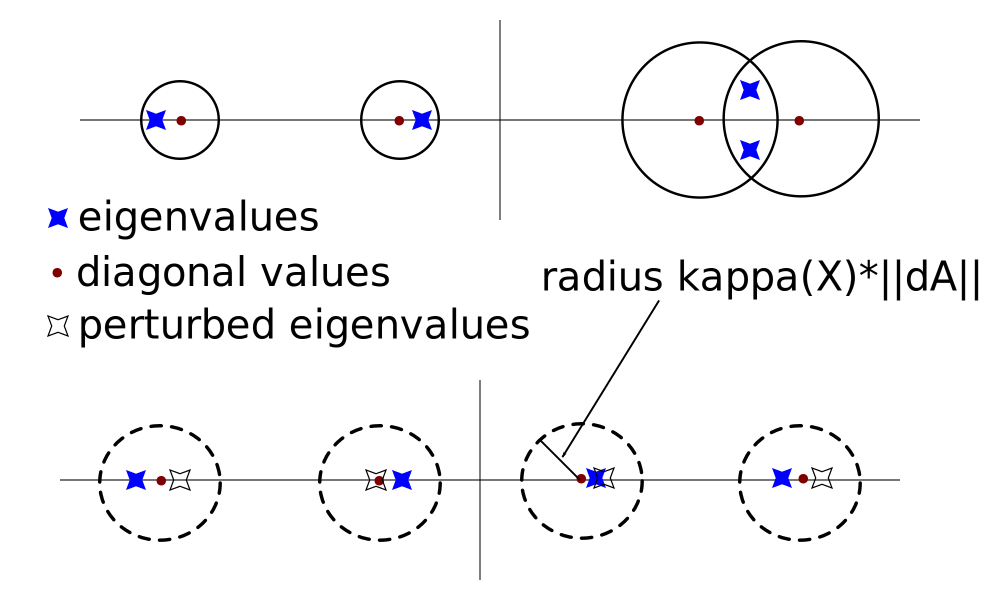
\includegraphics[width=3.5in]{diagrams/gershgorin}

}

\begin{itemize}
\item Top corresponds to Gershgorin disks on complex plane of 4-by-4 real matrix.
\item Bottom part corresponds to bounds on Gershgorin disks of $\B{X}^{-1} (\B A + \B{\delta A}) \B{X}$, which contain the eigenvalues $\B D$ of $\B A$ and the perturbed eigenvalues $\B D +\B{\delta D}$ of $\B A + \B{\delta A}$ provided that $||\B{\delta A}||$ is sufficiently small.
\end{itemize}

\end{frame}

%\begin{frame}{Gershgorin Theorem}
%
%\begin{itemize}
%\item Another way to show that the eigenvalues of a matrix are insensitive to perturbation is via Gershgorin theorem, which states that
%
%\lgcond{
% Given a matrix $\boldsymbol{A}\in{\mathbb{R}^{n\times{n}}}$, let $r_{i}=\sum_{j\neq{i}}|a_{ij}|$. We define the Gershgorin disks as
%$$
%    D_{i}=\{z\in{\mathbb{C}} : |z-a_{ii}|\leq{r_{i}} \}.
%$$
%}\lgcond{
%The eigenvalues $\lambda_1,\ldots,\lambda_n$ of any matrix $\boldsymbol{A}\in{\mathbb{R}^{n\times{n}}}$ are contained in the union of the Gershgorin disks,
%    $$
%        \forall i\in \{1,\ldots, n\}, \quad \lambda_i \in \bigcup_{j=1}^{n}{D_{j}}.
%    $$
%}
%\end{itemize}
%
%\end{frame}

\begin{frame}{Conditioning of Particular Eigenpairs}

\begin{itemize}
\item Consider the effect of a matrix perturbation on an eigenvalue $\lambda$ associated with a right eigenvector $\B x$ and a left eigenvector $\B y$, $\lambda = \B y^H \B A \B x / \B y^H \B x$

\lgcond{
For a sufficiently small perturbation $\B{\delta A}$, the eigenvalue $\lambda$ is perturbed to an eigenvalue $\hat{\lambda}$ of $\B{\hat{A}} = \B{A}+\B{\delta A}$.
The eigenvalue perturbation,
\[|\hat{\lambda}-\lambda| =  |\B y^H \B{\delta A} \B x / \B y^H \B x| \leq \frac{||\B{\delta A}||}{|\B y^H\B x|},\]
is small if $\B x$ is near-parallel to $\B y$ and large if they are near-perpendicular.
}

\item A more accurate eigenvalue approximation than Rayleigh quotient 
      for a normalized perturbed eigenvector (e.g. iterative guess) $\B{\hat{x}} = \B x+\B{\delta x}$,
      can be obtain with an estimate of both eigenvectors (also  $\B{\hat{y}} = \B y+\B{\delta y}$),
%Connect the notion of the angle between left and right eigenvectors to the magnitude of off-diagonal entries in the Schur form
\lgcond{
\begin{alignat*}{2}
|\hat{\lambda}_\text{xAx} - \lambda| &\approx |\B{\delta x}^H \B{A} \B{x} + \B{x}^H \B{A} \B{\delta x}| &&\leq |\lambda| ||\B{\delta x}|| + \Big(|\lambda| |\B{y}^H\B{x}| + |1-\B{y}^H\B{x}|\cdot ||\B A||\Big)||\B{\delta x}|| \\
|\hat{\lambda}_\text{yAx} - \lambda| &\approx \left|\frac{\B{\delta y}^H \B{A} \B{x} + \B{y}^H \B{A} \B{\delta x}}{\B{y}^H\B{x}}\right| &&\leq |\lambda| \frac{||\B{\delta x}|| + ||\B{\delta y}||}{|\B{y}^H\B{x}|}
\end{alignat*}
}

\end{itemize}

\end{frame}

\section{Basic Iterative Algorithms for Extremal Eigenpairs}

\begin{frame}{Power Iteration}
\urcornerlinkdemo{04-eigenvalues}{Power iteration and its Variants}

\begin{itemize}
\item \coloremph{Power iteration} can be used to compute the largest eigenvalue of a real symmetric matrix $\B A$:
\lgcond{
\[\B x^{(i)} = \B A \B x^{(i-1)} \quad \text{(typically with normalization of $\B x^{(i)}$ at each step)}.\]
For a random $\B x^{(0)}$, power iteration converges eigenvalue of $\B A$ with largest modulus,
\(\lim_{i\to \infty} \rho_{\B A}(\B x^{(i)}) = \lambda_\text{max}(\B A).\)
If this eigenvalue has multiplicity one, power iteration converges to \coloremph{dominant eigenvector}.
}

\item %Consider a real symmetric positive definite (SPD) $\B A$, then 
The error of power iteration decreases at each step by the ratio of the largest eigenvalues:

\lgcond{
%$\B A$ is SPD, so its eigenvalues are positive and eigenvectors $\B Q$ are orthonormal,
Assuming $\B A$ is diagonalizable with eigenvectors $\B U$ and $\B V^H = \B U^{-1}$,
\[\B x^{(k)} = \B A^k \B x^{(0)} = (\B U \B D \B V^{H})^k \B x^{(0)} = \B U \B D^k \B V^{H} \B x^{(0)} = \sum_{i=1}^n \B u_i\underbrace{\lambda_i^k \B v_i^H \B x^{(0)}}_{\alpha^{(i,k)}}.\]
The coefficient $\alpha^{(i,k)}$ associated with the maximum $\lambda_i$ and dominant eigenvector $\B u_i$ grows relatively, since $|\alpha^{(i,k)}/\alpha^{(j,k)}| = (|\lambda_{i}|/|\lambda_j|)^k\underbrace{|\alpha^{(i,0)}/\alpha^{(j,0)}|}_{\text{constant}}$.
}

\end{itemize}

\end{frame}

\begin{frame}{Inverse and Rayleigh Quotient Iteration}
\dblurcornerlinkinclass{inclass-eig}{Inverse Iteration with a Shift}{inclass-rayleigh}{Rayleigh Quotient Iteration}

\begin{itemize}
\item \coloremph{Inverse iteration} uses LU/QR/SVD of $\B A$ to run power iteration on $\B A^{-1}$

\lgcond{
\begin{itemize}
\item For a randomly chosen $\B x^{(0)}$, solving
\[\B A \B x^{(i)} = \B x^{(i-1)} \quad \text{(typically with normalization of $\B x^{(i)}$ at each step)}.\]
converges to $\lim_{i\to \infty} \rho_{\B A}(\B x^{(i)})=\lambda_\text{min}(\B A)$ provided there is a unique eigenvalue with minimum magnitude.
\sitem Inverse iteration on $\B A - \sigma \B I$ converges to the eigenvalue closes to $\sigma$, since all eigenvalues are shifted by $\sigma$.
\end{itemize}
}
\item \coloremph{Rayleigh quotient iteration} provides rapid convergence to an eigenpair
\lgcond{
\[(\B A-\rho_{\B A}(\B x^{(i-1)})\B I) \B x^{(i)} = \B x^{(i-1)},\]
since at each step the relative magnitude largest eigenvalue of $(\B A-\rho_{\B A}(\B x^{(i-1)})\B I)^{-1}$ grows.
Formally, it achieves cubic convergence, but requires matrix refactorization at each step.
}
\end{itemize}

\end{frame}

\section{Algorithms for Finding Many Eigenpairs}

\subsection{Deflation}

\begin{frame}{Deflation}

\begin{itemize}
\item Power, inverse, and Rayleigh-quotient iteration compute a single eigenpair, to obtain further eigenpairs, can perform \coloremph{deflation}

\lgcond{
\begin{itemize}
\sitem Given eigenvalue $\lambda_1$ and right eigenvector $\B x_1$, seek $\B v$ so that $\B B = \B A-\lambda_1 \B u \B v^T$ has eigenvalues $\lambda_2,\ldots,\lambda_n$, where
\[\B A = \B X \B D \underbrace{\B Y^T}_{\B X^{-1}} = \sum_{i=1}^n\lambda_i\B x_i\B y_i^T.\]
\sitem Ideal choice would be $\B v = \B y_1^T$, i.e. the left eigenvector associated with $\lambda_1$, as then the $n-1$ other eigenvectors of  $\B B$ would be the same as those of $\B A$.
\sitem For symmetric matrices $\B y_1 =\B x_1$, but for nonsymmetric, obtaining $\B y_1$ may require more work.
\sitem Good alternative choice for nonsymmetric is to select $\B v = \B x_1$, as then the Schur vectors are unmodified, since for $\B A = \B Q \B T \B Q^T$, with $t_{11}=\lambda_1$, $\B q_1= \B x_1$, we get
\[\B B = \B Q \B T \B Q^T -\lambda_1 \B q_1 \B q_1^T= \B Q(\B T - \lambda_1 \B Q^T\B q_1 \B q_1^T \B Q)\B Q^T= \B Q (\B T - \lambda_1 \B e_1\B e_1^T)\B Q^T.\]

\end{itemize}
}
\lgcond{}
\end{itemize}

\end{frame}

%\begin{frame}{Eigenvalues and the Field of Values}
%
%\begin{itemize}
%\item The field of values is the set of possible Rayleigh quotients of matrix $\B A$:
%
%\lgcond{
%\[W(\B A)=\{\rho_{\B A}(\B x) : \B x \in\mathbb{C}^n\}\]
%}
%
%
%\item If and only if the matrix is normal, the field of values is the convex hull of the eigenvalues:
%
%\lgcond{
%For \(\B A = \B X \B D \B X^{-1}\) 
%\begin{itemize}
%\item
%all eigenvalues are in the field of values, 
%$\forall i, d_{ii} \in W(\B A)$.
%\item if the matrix is normal, \(\B X ^{-1} = \B X^T\), 
%\[W(\B A) = \Big\{s : s=\sum_{i=1}^n x_id_{ii}, ||\B{x}||_1\leq 1\Big\}\]
%\end{itemize}
%}
%
%\end{itemize}
%
%\end{frame}

\subsection{Reduction to Hessenberg}

\begin{frame}{Direct Matrix Reductions}
\urcornerlinkdemo{04-eigenvalues}{Householder Similarity Transforms}

\begin{itemize}
\item We can always compute an orthogonal similarity transformation to reduce a general matrix to \coloremph{upper-Hessenberg} (upper-triangular plus the first subdiagonal) matrix $\B H$, i.e. $\B A = \B Q \B H \B Q^T$:

\lgcond{
We can perform successive two-sided application of Householder reflectors
\[\B A =\begin{bmatrix} h_{11} & a_{12} & \cdots \\ a_{21} & a_{22} &  \\ \vdots & &\ddots  \end{bmatrix}  = \textcolor{darkred}{\B{Q}_1} \begin{bmatrix} h_{11} & a_{12} & \cdots \\ \textcolor{darkred}{h_{21}} & \textcolor{darkred}{t_{22}} &  \textcolor{darkred}{\cdots} \\ \textcolor{darkred}{\B{0}} & \textcolor{darkred}{\vdots} &\textcolor{darkred}{\ddots}  \end{bmatrix}  = \B{Q}_1  \begin{bmatrix} h_{11} & \textcolor{darkred}{h_{12}} & \textcolor{darkred}{\cdots} \\ h_{21} & \textcolor{darkred}{h_{22}} &  \textcolor{darkred}{\cdots} \\ \B{0} & \textcolor{darkred}{\vdots} &\textcolor{darkred}{\ddots}  \end{bmatrix}\textcolor{darkred}{\B{Q}_1^T}=\cdots\]
subsequent columns can be reduced by induction, so we can always stably reduce to upper-Hessenberg with roughly the same cost as QR.
}

\item In the symmetric case, Hessenberg form implies tridiagonal:

\lgcond{
If $\B{A}=\B{A}^T$ then $\B{H}=\B{Q}\B{A}\B{Q}^T=\B{H}^T$, and a symmetric upper-Hessenberg matrix must be tridiagonal.
}

\end{itemize}

\end{frame}

\subsection{Orthogonal Iteration}

\begin{frame}[fragile]{Simultaneous and Orthogonal Iteration}
\urcornerlinkdemoinclass{04-eigenvalues}{Orthogonal Iteration}{inclass-orthogonal-iteration}{Orthogonal Iteration}

\begin{itemize}
\item \coloremph{Simultaneous iteration} provides the main idea for computing many eigenvectors at once:

\lgcond{
\begin{itemize}
\sitem Initialize $\B X_0\in \mathbb{R}^{n \times k}$ to be random and perform
\[\B X_{i+1} = \B A \B X_i.\]
\item Observe that $\lim_{i\to \infty} \text{span}(\B X_{i}) = \mathbb{S}$ where $\mathbb{S}$ is the subspace spanned by the $k$ eigenvectors of $\B A$ with the largest eigenvalues in magnitude.
\sitem Can use this to compute the right singular vectors of matrix $\B M$ by using $\B A = \B M^T \B M$ (no need to form $\B A$, just multiply $\B X_i$ by $\B M^T$ then $\B M$).
\sitem Small number of iterations suffice to obtain reasonable low-rank approximation of $\B M$, and ultimately $\B X$ converge to singular vectors in truncated SVD.
\end{itemize}
} 

\item Orthogonal iteration performs QR at each step to ensure stability 

\vspace*{-.5cm}
\lgcond{
\[\B{Q}_{i+1}\B{R}_{i+1}=\B{A}\B{Q}_{i}\]
\vspace*{-.5cm}
\begin{itemize}
\item $\B{Q}_i$ has the same span as $\B X_{i}$ in orthogonal iteration.
\sitem QR has cost $O(nk^2)$ while product has cost $O(n^2k)$ per iteration.
\end{itemize}
}
\end{itemize}
\end{frame}

\subsection{QR Iteration}

\begin{frame}{QR Iteration}

\begin{itemize}
\item QR iteration reformulates orthogonal iteration for $n=k$ to reduce cost/step,

\lgcond{
\begin{itemize}
\item Orthogonal iteration computes $\B{\textcolor{darkred}{\hat{Q}}}_{i+1}\B{\textcolor{darkred}{\hat{R}}}_{i+1}=\B{A}\B{\textcolor{darkred}{\hat{Q}}}_{i}$
\sitem QR iteration computes $\B{A}_{i+1} =\B{R}_i\B{Q}_i$  at iteration $i$ %$ = \B{\textcolor{darkred}{\hat{Q}}}_{i+1}^T\B A \B{\textcolor{darkred}{\hat{Q}}}_{i+1}$
\end{itemize}

}

\item Using induction, we assume $\B{A}_{i}= \B{\textcolor{darkred}{\hat{Q}}}_{i}^T\B A \B{\textcolor{darkred}{\hat{Q}}}_{i}$ and show that QR iteration obtains $\B{A}_{i+1}= \B{\textcolor{darkred}{\hat{Q}}}_{i+1}^T\B A \B{\textcolor{darkred}{\hat{Q}}}_{i+1}$
\lgcond{
\begin{itemize}
\sitem QR iteration performs QR to obtain $\B{Q}_i\B{R}_i = \B{A}_i$
\sitem Orthogonal iteration performs QR
\[\B{\textcolor{darkred}{\hat{Q}}}_{i+1}
  \B{\textcolor{darkred}{\hat{R}}}_{i+1}
  =\B A \B{\textcolor{darkred}{\hat{Q}}}_{i}
  \underbrace{=}_{\text{inductive assumption}}
   \B{\textcolor{darkred}{\hat{Q}}}_{i}\B A_i 
  =\underbrace{\B{\textcolor{darkred}{\hat{Q}}}_{i}\B{Q}_i}_{\B{\textcolor{darkred}{\hat{Q}}}_{i+1}}\underbrace{\B{R}_i}_{\B{\textcolor{darkred}{\hat{R}}}_{i+1}}\]
consequently, we can observe that $\B{R}_i = \underbrace{\B{Q}_i^T \B{\textcolor{darkred}{\hat{Q}}}_{i}^T}_{\B{\textcolor{darkred}{\hat{Q}}}_{i+1}^T} \B A \B{\textcolor{darkred}{\hat{Q}}}_{i}$
%$$ so $ \B{A} = \B{\textcolor{darkred}{\hat{Q}}}_{i+1}\B{\textcolor{darkred}{\hat{R}}}_{i+1}\B{\textcolor{darkred}{\hat{Q}}}_{i}^T$
\sitem QR iteration performs product 
$\B{A}_{i+1}=\B R_i \B Q_i = \B{\textcolor{darkred}{\hat{Q}}}_{i+1}^T \B A \B{\textcolor{darkred}{\hat{Q}}}_{i+1}$
%$$ = \B{\textcolor{darkred}{\hat{R}}}_{i+1} \B{\textcolor{darkred}{\hat{Q}}}_{i}^T\B{\textcolor{darkred}{\hat{Q}}}_{i+1} = \B{R}_{i} \B{Q}_{i}$$
\end{itemize}

}
%\item Show that similarity transformations are being performed

\lgcond{}

\end{itemize}

\end{frame}

\begin{frame}{QR Iteration with Shift}
\urcornerlinkinclass{inclass-qr-iteration}{QR Iteration}

\begin{itemize}
\item QR iteration can be accelerated using shifting:
\lgcond{
\begin{align*}
\B{Q}_i\B{R}_i &= \B{A}_i - \sigma_i\B I \\
\B{A}_{i+1} &= \B{R}_i\B{Q}_i + \sigma_i\B I 
\end{align*}
note that $\B{A}_{i+1}$ is similar to $\B{A}_i$, since we can reorganize the above as 
\begin{align*}
\B{R}_i\B{Q}_i &= \B{Q}_i^T(\B{A}_i - \sigma_i\B I) \B{Q}_i,\\
 \B{Q}_i(\B{A}_{i+1} - \sigma_i\B I)\B Q_i^T &= \B{Q}_i\B{R}_i, 
\end{align*}
and observe that $\B{R}_i\B{Q}_i$ is similar to $\B{Q}_i\B{R}_i$.
}

\sitem The shift is typically selected to accelerate convergence with respect to a particular eigenvalue:

\lgcond{
We can select the shift as the bottom right element of $\B{A}_i$, which would be the smallest eigenvalue if $\B{A}_i$ is triangular (we have converged). 
Such shifting should accelerate convergence of the last column of $\B{A}_i$, once finished we should operate only on the first $n-1$ columns, and so on.
}

\end{itemize}

\end{frame}

%\begin{frame}{Hessenberg and Tridiagonal Form}
%
%\begin{itemize}
%\item Describe reduction to Hessenberg form
%
%\lgcond{
%QR provides us with a way to reduce a matrix to triangular form by an orthogonal transformation.
%For the eigenvalue problem, we wish to perform similarity transformations, which need to be applied from both sides.
%Note that if simply compute the QR factorization of the first panel of $\B A=[\B{A}_1, \B{A}_2]$, $\B{A}_1=\B{Q}\B{R}$, then $\B{Q}^T \B A\B{Q}$ is still generally dense $\B{Q}^T\B A$ has at least as many zeros as in $\B{R}$.
%However, we can use QR factorization to introduce zeros by similarity transformation via
%\[\begin{bmatrix} \B{A}_{11} & \B{A}_{12} \\ \B{A}_{21} & \B{A}_{22} \end{bmatrix} = \begin{bmatrix} \B{A}_{11} & \B{A}_{12} \\ \B{Q}\B{R} & \B{A}_{22} \end{bmatrix} =\begin{bmatrix} \B I & \\ & \B{Q} \end{bmatrix}\begin{bmatrix} \B{A}_{11} & \B{A}_{12}\B{Q} \\ \B{R} & \B{Q}^T\B{A}_{22}\B{Q} \end{bmatrix}\begin{bmatrix} \B I & \\ & \B{Q}^T\end{bmatrix}\]
%if we pick $\B{A}_{11}$ to be $1\times 1$ then doing this for each panel will yield an upper-Hessenberg result. 
%}
%
%\item Describe reduction to tridiagonal form in symmetric case
%
%\lgcond{
%In the symmetric case $\B{A}_{12}\B{Q}=\B{A}_{21}^T\B{Q}=(\B{Q}^T\B{A}_{21})^T=\B{R}^T$, so we reduce to a banded (tridiagonal if $\B{A}_{11}$ is $1\times 1$) matrix.
%}
%
%\end{itemize}
%
%\end{frame}

\begin{frame}{QR Iteration Complexity}

\begin{itemize}
\item  QR iteration is accelerated by first reducing to upper-Hessenberg or tridiagonal form:

\lgcond{
Reduction to upper-Hessenberg or tridiagonal in the symmetric case, costs $O(n^3)$ operations and can be done in a similar style to Householder QR. \\
\ \\
Given an upper-Hessenberg matrix, $\B H_i=\B A_i$ 
\begin{itemize} 
\item reduction to upper-triangular requires $n-1$ Givens rotations, if $\B G_i$ rotates the $(i+1)$th row into the $i$th to eliminate the $i$th element on the first subdiagonal,
  \(\B R_i = \B G_{1}^T\cdots \B G_{n-1}^T\B H_i\)
\mitem computation of $\B H_{i+1} = \B R \B Q$ can be done by application of the $n-1$ Givens rotations to $\B R$ from the right $\B H_{i+1} = \B R_i \B G_{n-1}\cdots \B G_{1}$.
\end{itemize}
Both cost $O(n^2)$, for $O(n^3)$ overall if QR iteration converges in $O(n)$ steps.
}

\lgcond{
Given a tridiagonal matrix, the same two general steps are required, but now each step costs $O(n)$, so overall the eigenvalues and eigenvectors of a tridiagonal matrix can be computed with $O(n^2)$ work.
}

\end{itemize}

\end{frame}


%\begin{frame}{Solving Hessenberg Nonsymmetric Eigenproblems}
%
%\begin{itemize}
%\item Eigenvalues of a Hessenberg matrix are usually computed by QR iteration:
%
%\lgcond{
%Using $\B{A}_0=\B{H}$, with a shift of $\sigma_i$ at iteration $i$ QR iteration is
%\begin{align*}
%\B{Q}_i\B{R}_i &= \B{A}_i - \sigma_i\B I \\
%\B{A}_{i+1} &= \B{R}_i\B{Q}_i + \sigma_i\B I 
%\end{align*}
%
%}
%
%\item Good convergence guarantees given by Francis (Wilkinson) shift:
%
%\lgcond{
%To handle complex eigenvalues, diagonalize the bottom-right 2-by-2 block of $\B{A}_{i}$ and use the eigenvalues $\sigma_i,\bar{\sigma}_i$ as the next two shifts (also possible to reorganize and do a double-step with two shifts).
%
%}
%
%\end{itemize}
%
%\end{frame}

\section{Tridiagonal Eigenproblems}

\begin{frame}{Solving Tridiagonal Symmetric Eigenproblems}

A variety of methods exists for the tridiagonal eigenproblem:
\begin{itemize}
\item QR iteration \smcond{requires $O(1)$ QR factorizations per eigenvalue, $O(n^2)$ cost to get eigenvalues, $O(n^3)$ for eigenvectors. The last cost is not optimal.}



\item Divide and conquer
\lgcond{}
\lgcond{reduces tridiagonal $\B{T}$ by a similarity transformation to a rank-1 perturbation of identity, then computes its eigenvalues using roots of secular equation
\begin{align*}
\B{T} &= \begin{bmatrix} \B{T}_1 & t_{n/2+1,n/2}\B{e}_{n/2}\B{e}^T_{1} \\ t_{n/2+1,n/2}\B{e}_{1} \B{e}_{n/2}^T& \B{T}_2 \end{bmatrix} \\
&= \begin{bmatrix} \B{\hat{T}}_1 &  \\ & \B{\hat{T}}_2 \end{bmatrix} + t_{n/2+1,n/2}\begin{bmatrix} \B{e}_{n/2} \\ \B{e}_{1} \end{bmatrix} \begin{bmatrix} \B{e}_{n/2}^T & \B{e}_{1}^T \end{bmatrix}
= \begin{bmatrix} \B{Q}_1\B{D}_1\B{Q}_1^T &  \\ & \B{Q}_2\B{D}_2\B{Q}_2^T \end{bmatrix} + \ldots \\
&=\begin{bmatrix} \B{Q}_1 & \\ & \B{Q}_2\end{bmatrix} \bigg(\underbrace{\begin{bmatrix} \B{D}_1 &  \\ & \B{D}_2 \end{bmatrix}
+ t_{n/2+1,n/2}\begin{bmatrix} \B{Q}_{1}^T\B{e}_{n/2} \\ \B{Q}_2^T\B{e}_{1} \end{bmatrix} \begin{bmatrix} \B{e}_{n/2}^T\B{Q}_1 & \B{e}_{1}^T\B{Q}_2 \end{bmatrix}}_{\B{D}+\alpha \B{u}\B{u}^T}\bigg)\begin{bmatrix} \B{Q}_1^T & \\ & \B{Q}_2^T\end{bmatrix}
\end{align*}
}

\end{itemize}

\end{frame}

\begin{frame}[fragile]{Solving the Secular Equation for Divide and Conquer}

To solve the eigenproblem at each step, the divide and conquer method needs to diagonalize a rank-1 perturbation of a diagonal matrix
\[\B{A} = \B{D} + \alpha \B{u}\B{u}^T.\]
\lgcond{
\begin{itemize}
\item The zeros of the characteristic polynomial define the eigenvalues,
\[f(\lambda) =\text{det}(\B D + \alpha \B u \B u^T- \lambda \B I )=1+\alpha\B u^T (\B D - \lambda \B I)^{-1}\B u=1+\alpha\sum_{i=1}^n\frac{u_i^2}{d_{ii}-\lambda}=0.\]
\item This nonlinear equation can be solved efficiently by a variant of Newton's method (covered in the next chapter) 
      that uses hyperbolic rather than linear extrapolations at each step.
\sitem Major alternatives to divide and conquer include spectral bisection and the MRRR algorithm.
\end{itemize}
}
\lgcond{}
\end{frame}

%\begin{frame}{Solving Tridiagonal Symmetric Eigenproblems (II)}
%
%\begin{itemize}
%\item Jacobi iteration
%\mdcond{uses two-sided Givens rotations, to introduce zeros, typically by eliminating the largest value in magnitude, requires $O(1)$ sweeps over all nonzeros, $O(n^2)$ cost to get eigenvalues, $O(n^3)$ to get eigenvectors.}
%
%\item Bisection
%\lgcond{finds a partition point using $\B L\B D\B L^T$ factorization or Sturm sequence to compute inertia (\#positive eigenvalues, \#negatives eigenvalues, \#zero eigenvalues). Sylvester's inertia theorem shows that inertia is preserved under any transformation $\B A = \B S \B B \B S^T$ where $\B S$ is an invertible matrix.
%Consequently, the diagonal $\B D$ matrix in the $\B L \B D \B L^T$ factorization has the same inertia as $\B A$.
%Computing this factorization with various shifts enables successive halving of the approximation interval.
%}
%
%\item Relatively robust representation (RRR and MRRR)
%\mdcond{leverages stability of values in $\B L\B D\B L^T$ and other techniques to compute all eigenvectors and eigenvalues in $O(n^2)$ cost. 
%These factorized forms minimize sensitivity to round-off error.}
%
%\end{itemize}
%
%\end{frame}


\section{Krylov Subspace Methods}

\subsection{Krylov Subspaces}

\begin{frame}{Introduction to Krylov Subspace Methods}

\begin{itemize}
\item \coloremph{Krylov subspace methods} work with information contained in the $n\times k$ matrix 
\[\B{K}_k=\begin{bmatrix} \B{x_0} & \B A\B{x_0} & \cdots & \B A^{k-1}\B{x_0}\end{bmatrix}\]

\mdcond{
We seek to best use the information from the matrix vector product results (columns of $\B{K}_k$) to solve eigenvalue problems.
}

\item The matrix $\B{K}_n^{-1}\B{A}\B{K}_n$ is a \coloremph{companion matrix} $\B C$:

\mdcond{
Letting $\B{k}^{(i)}_n = \B{A}^{i-1}\B{x}$, we observe that
%$\B{K}_n=\begin{bmatrix} \B{k}^{(1)}_n & \cdots & \B{k}^{(n)}_n\end{bmatrix}$ observe that 
\[\B{A}\B{K}_n= \begin{bmatrix} \B A \B{k}^{(1)}_n & \cdots & \B A \B{k}^{(n-1)}_n& \B A \B{k}^{(n)}_n\end{bmatrix}= \begin{bmatrix} \B{k}^{(2)}_n & \cdots & \B{k}^{(n)}_n & \B{A}\B{k}^{(n)}_n\end{bmatrix},\]
therefore premultiplying by $\B{K}_m^{-1}$ transforms the first $n-1$ columns of $\B{A}\B{K}_n$ into the last $n-1$ columns of $\B{I}$,
\begin{align*}
\B{K}_n^{-1}\B{A}\B{K}_n&= \begin{bmatrix} \B{K}_n^{-1}\B{k}^{(2)}_n & \cdots & \B{K}_n^{-1}\B{k}^{(n)}_n & \B{K}_n^{-1}\B{A}\B{k}^{(n)}_n\end{bmatrix} \\
&=\begin{bmatrix} \B{e}_2 & \cdots & \B{e}_n & \B{K}_n^{-1}\B{A}\B{k}^{(n)}_n\end{bmatrix}
\end{align*}
}
\lgcond{}

\end{itemize}

\end{frame}

\begin{frame}{Krylov Subspaces}

\begin{itemize}
\item Given $\B Q_k \B R_k = \B{K}_k$, we obtain an orthonormal basis for the Krylov subspace,
      
\[\mathcal{K}_k(\B A, \B x_0)=\mathop{span}(\B Q_k)= \{p(\B A)\B{x}_0 : \mathop{deg}(p) < k\},\]
where $p$ is any polynomial of degree less than $k$.

\sitem The Krylov subspace includes the $k-1$ approximate dominant eigenvectors generated by $k-1$ steps of power iteration:


\lgcond{
\begin{itemize}
\item The approximation obtained from $k-1$ steps of power iteration starting from $\B{x}_0$ is given by the Rayleigh-quotient of $\B{y}=\B{A}^k\B{x}_0$. 
\sitem This vector is within the Krylov subspace, $\B{y}\in\mathcal{K}_k(\B A, \B x_0)$.
\sitem Consequently, Krylov subspace methods will generally obtain strictly better approximations of the dominant eigenpair than power iteration.
\end{itemize}
}
\lgcond{}

\end{itemize}

\end{frame}


\subsection{Ritz Values and Vectors}

\begin{frame}{Krylov Subspace Methods}

\begin{itemize}
\item The $k\times k$ matrix $\B H_k = \B Q_k^T\B A \B Q_k$ minimizes $||\B A \B Q_k - \B Q_k \B H_k||_2$:

\lgcond{
The minimizer $\B X$ for the linear least squares problem $\B{Q}_k\B{X} \cong \B{A}\B{Q}_k$ is (via the normal equations) $\B{X}=\B{Q}_k^T\B{A}\B{Q}_k=\B{H}_k$.

}

\item $\B H_k$ is Hessenberg, because the companion matrix $\B C_k$ is Hessenberg:

\lgcond{
\[\B H_k = \B Q_k^T\B A \B Q_k = \B{R}_k\B{K}_k^{-1} \B{A} \B{K}_k \B{R}_k^{-1} =  \B{R}_k\B{C}_k \B{R}_k^{-1}\]
is a product of three matrices: upper-triangular $\B R_k$, upper-Hessenberg $\B C_k$ , and upper-triangular $\B R^{-1}_k$, which results in upper-Hessenberg $\B H_k$.
}

\end{itemize}

\end{frame}


\begin{frame}{Rayleigh-Ritz Procedure}

\urcornerlinkdemoinclass{04-eigenvalues}{Arnoldi vs Power Iteration}{inclass-ritz}{Computing the Maximum Ritz Value}

\begin{itemize}
\item The eigenvalues/eigenvectors of $\B{H}_k$ are the \coloremph{Ritz values/vectors}:

\mdcond{
\[\B{H}_k=\B{X}\B{D}\B{X}^{-1}\]
eigenvalue approximations based on Ritz vectors $\B{X}$ are given by $\B{Q}_k\B{X}$.
}

\item The Ritz vectors and values are the \coloremph{ideal approximations} of the actual eigenvalues and eigenvectors based on only $\B{H}_k$ and $\B{Q}_k$:

\lgcond{
Assuming $\B A$ is a symmetric matrix with positive eigenvalues, the largest Ritz value $\lambda_\text{max}(\B H_k)$ will be the maximum Rayleigh quotient of any vector in $\mathcal{K}_k=\mathop{span}(\B{Q}_k)$,
\[\max_{\B x\in \mathop{span}(\B{Q}_k)}\frac{\B{x}^T\B A \B x}{\B x^T \B x} = \max_{\B y\neq 0}\frac{\B{y}^T\B{Q}_k^T\B A \B{Q}_k \B y}{\B y^T \B y} =\max_{\B y\neq 0}\frac{\B{y}^T\B{H}_k \B y}{\B y^T \B y}=\lambda_\text{max}(\B H_k),\]
which is the best approximation to $\lambda_\text{max}(\B A) = \max_{\B x\neq 0}\frac{\B{x}^T\B{A} \B x}{\B x^T \B x}$ available in $\mathcal{K}_k$.
The quality of the approximation can also be shown to be optimal for other eigenvalues/eigenvectors.
}

\end{itemize}

\end{frame}

\subsection{Arnoldi Algorithm}

\begin{frame}{Arnoldi Iteration}

\dblurcornerlinkdemo{04-eigenvalues}{Arnoldi Iteration}{04-eigenvalues}{Arnoldi Iteration with Complex Eigenvalues}
\begin{itemize}
\item Arnoldi iteration computes $\B{H}=\B{H}_n$ directly using the recurrence $\B{q}^T_i\B{A}\B{q}_j=h_{ij}$, where $\B q_l$ is the $l$th column of $\B Q_n$:

\lgcond{
We have that 
\[\B{q}^T_i\B{A}\B{q}_j=\B{q}^T_i(\B{Q}_n\B{H}_n\B{Q}_n^T)\B{q}_j = \B{e}_i^T\B{H}_n\B{e}_j=h_{ij}.\]
}

\item After each matrix-vector product, orthogonalization is done with respect to each previous vector:

\lgcond{
Given $\B{u}_j=\B{A}\B{q}_j$, compute $h_{ij}=\B{q}_i^T\B{u}_j$ for each $i\leq j$, forming a column of the $\B H$ matrix at a time.
}


\end{itemize}

\end{frame}

\subsection{Lanczos Algorithm}

\begin{frame}{Lanczos Iteration}

\urcornerlinkinclass{inclass-eig-methods-for-low-rank}{Approximation with Orthogonal Iteration and Lanczos}

\begin{itemize}
\item Lanczos iteration provides a method to reduce a symmetric matrix to a tridiagonal matrix: 

\lgcond{
Arnoldi iteration on a symmetric matrix will result in an upper-Hessenberg matrix $\B H_n$ as before, except that it must also be symmetric, since
\[\B{H}_n^T=(\B{Q}_n^T\B{A}\B{Q}_n)^T = \B{Q}_n^T\B{A}^T\B{Q}_n=\B{Q}_n^T\B{A}\B{Q}_n=\B{H}_n,\]
which implies that $\B{H}_n$ must be tridiagonal.
}

\item After each matrix-vector product, it suffices to orthogonalize with respect to two previous vectors:

\lgcond{
Since $h_{ij}=0$ if $|i-j|>1$, given $\B{u}_j=\B{A}\B{q}_j$, it suffices to compute only $h_{jj}=\B{q}_j^T\B{u}_j$ and $h_{j-1,j}=h_{j,j-1}=\B{q}_{j-1}^T\B{u}_j$.
}

\end{itemize}


\end{frame}

\subsection{Computational Cost}

\begin{frame}{Cost Krylov Subspace Methods}

\begin{itemize}
\item The cost of matrix-vector multiplication when the matrix has $m$ nonzeros
\lgcond{
is $m$ multiplications and at most $m$ additions, so roughly $2m$ in total.
}

\item The cost of orthogonalization at the $k$th iteration of a Krylov subspace method is
\lgcond{
\begin{itemize}
\sitem $O(nk)$ for $k$ inner products in Arnoldi, 
\sitem $O(n)$ in Lanczos, since only 2 orthogonalizations needed.
\sitem For Arnoldi with $k$-dimensional subspace, orthogonalization costs $O(nk^2)$, matrix-vector products cost $O(mk)$, so generally desire $nk<m$.
\end{itemize}
}


\end{itemize}

\end{frame}

\subsection{Restarting}

\begin{frame}{Restarting Krylov Subspace Methods}

\begin{itemize}
\item In finite precision, Lanczos generally loses orthogonality, while orthogonalization in Arnoldi can become prohibitively expensive:

\lgcond{
\begin{itemize} 
\item Arnoldi cost of orthogonalization dominates if $k>m/n$.
\item In Lanczos, reorthogonalizing iterate to previous guesses can ensure orthogonality.
\item Selective orthogonalization strategies control when and with respect to what previous columns of $\B{Q}$, each new iterate $\B{u}_j=\B{A}\B{q}_j$ should be orthogonalized.
\end{itemize}

}

\item Consequently, in practice, low-dimensional Krylov subspace methods are constructed repeatedly using carefully selected new starting vectors:

\lgcond{
If we wish to find a particular eigenvector isolate some eigenspaces, restarting is beneficial
\begin{itemize}
\item can orthogonalize to previous eigenvector estimates to perform deflation,
\item can pick starting vector as Ritz vector estimate associated with desired eigenpair,
\item given new starting vector, can discard previous Krylov subspace, which helps make storing the needed parts of $\B{Q}$ possible.
\end{itemize}
}


\end{itemize}

\end{frame}
%
%\begin{frame}{Convergence of Lanczos Iteration}
%
%\begin{itemize}
%
%\item Cauchy interlacing theorem: eigenvalues of $\B{H}_k$, $\tilde{\lambda}_1\geq \cdots \geq \tilde{\lambda}_n$ with respect to eigenvalues of $\B{A}$, $\lambda_1 \geq \cdots \geq \lambda_n$ satisfy 
%\[\lambda_i \leq \tilde{\lambda_i} \leq \lambda_{n-k+i}\]
%
%\lgcond{}
%
%\item Convergence to extremal eigenvalues is generally fastest
%
%\lgcond{}
%
%\end{itemize}
%
%\end{frame}


%\begin{frame}{Applications of Eigenvalue Problems: Matrix Functions}
%
%
%\begin{itemize}
%\item Given $\B{A} = \B{X} \B{D}\B{X}^{-1}$ how can we compute $\B{A}^k$?
%\lgcond{
%\begin{align*}
%\B{A}^2 &= \B{X} \B{D}\B{X}^{-1}\B{X} \B{D}\B{X}^{-1} \\
%        &= \B{X} \B{D}^2\B{X}^{-1}, \\
%\B{A}^k &= \B{X} \B{D}^k\B{X}^{-1} 
%\end{align*}
%}
%\item What about $e^{\B{A}}$ ? 
%     $\log(\B{A})$? generally $f(\B{A})$?
%\lgcond{
%\begin{align*}
%e^{\B{A}} &= \B I + \B A + \B A / 2! + \cdots \\
%          &= \B X ( \B I + \B D + \B D^2/2! +\cdots ) \B X^{-1} \\
%          &= \B X e^{\B D} \B X^{-1} \\
%\log (\B A) &= \B X \log (\B D) \B X^{-1} \\
%f(\B A) &= \B X f(\B D) \B X^{-1}
%\end{align*}
%}
%
%\end{itemize}
%
%
%\end{frame}
%
%\begin{frame}{Applications of Eigenvalue Problems: Differential Equations}
%
%
%\begin{itemize}
%\item Consider solutions to an ordinary differential equation of the form $\B{\frac{dx}{dt}}(t) = \B{A}\B{x}(t) +\B{f}(t)$ with $\B{x}(0)=\B{x_0}$:
%
%$$\B x(t) = e^{t\B{A}}\B{x}_0 + \int_0^t e^{(t-\tau)\B{A}}\B{f}(\tau) d\tau$$
%
%\lgcond{}
%
%\item Using $\B{A}=\B{X}\B{D}\B{X}^{-1}$ permits us to compute the solution explicitly (Jordan form also suffices if $\B{A}$ is defective):
%
%\lgcond{
%$$\B x(t) = \B X e^{t\B{D}}\B{X}^{-1}\B{x}_0 + \B{X}\int_0^t e^{(t-\tau)\B{D}}\B{X}^{-1}\B{f}(\tau) d\tau$$
%}
%
%
%\end{itemize}
%
%
%\end{frame}
%
%\begin{frame}{Differential Equations using the Generalized Eigenvalue Problem}
%
%
%\begin{itemize}
%\item Consider a more general linear differential equation of the form $\B{B}\B{\frac{dx}{dt}}(t) = \B{A}\B{x}(t) +\B{f}(t)$ with $\B{x}(0)=\B{x_0}$, which we can reduce to the usual form by premultiplying with $\B{B}^{-1}$:
%% ($\B A$ can represent stiffness matrix and $\B B$ mass matrix):
%\lgcond{
%\[\B{\frac{dx}{dt}}(t) = \B{B}^{-1}\B{A}\B{x}(t) +\B{B}^{-1}\B{f}(t)\]
%However, $\B B $ may not be invertible and $\B{B}^{-1}\B{A}$ is generally nonsymmetric even when $\B B^{-1}$ and $\B A$ are.
%}
%
%\item If we can find $\B{X}$ such that $\B{A}=\B{X}\B{D_A}\B{X}^{-1}$  and $\B{B} = \B{X}\B{D_B}\B{X}^{-1}$ we could solve this equation while preserving symmetry of $\B{A}$ and $\B{B}$: 
%\lgcond{
%\begin{align*}
%\B x(t) &= e^{t\B{B}^{-1}\B{A}}\B{x}_0 + \int_0^t e^{(t-\tau)\B{B}^{-1}\B{A}}\B{f}(\tau) d\tau \\
% &= e^{t\B{X}\B{D_B}^{-1}\B{D_A}\B{X}^{-1}}\B{x}_0 + \int_0^t e^{(t-\tau)\B{X}\B{D_B}^{-1}\B{D_A}\B{X}^{-1}}\B{f}(\tau) d\tau \\
%&= \B{X}e^{t\B{D_B}^{-1}\B{D_A}}\B{X}^{-1}\B{x}_0 + \B{X} \int_0^t e^{(t-\tau)\B{D_B}^{-1}\B{D_A}}\B{X}^{-1}\B{f}(\tau) d\tau
%%\B{X}\B{D_B}\B{X}^{-1}\B{\frac{dx}{dt}}(t) &= \B{X}\B{D_A}\B{X}^{-1}\B{x}(t) +\B{f}(t) \\
%%\B{D_B}\B{D_A}^{-1}\B{y} \B{\frac{dy}{dt}}(t) &= \B{y}(t) +\B{X}^{-1}\B{f}(t), \quad \B y(t) = \B{D_A}\B{X}^{-1}\B{x}(t) 
%\end{align*}
%
%}
%
%
%\end{itemize}
%
%
%\end{frame}



\section{Generalized Eigenvalue Problems}

\begin{frame}{Generalized Eigenvalue Problem}


\begin{itemize}
\item
A generalized eigenvalue problem has the form $\B A \B x = \lambda \B B \B x$, 
\lgcond{
\begin{align*}
\B A \B X &= \B B \B X \B D \\
\B B^{-1} \B A &=  \B X \B D \B X^{-1} 
\end{align*}
Generalized eigenvalue problems arise frequently, especially in solving partial differential equations.
}
\item
When $\B A$ and $\B B$ are symmetric and $\B B$ is SPD, we can perform Cholesky on $\B{B}$, multiply $\B{A}$ by the inverted factors, and diagonalize it:
\lgcond{
\begin{align*}
\B A \B X &= \B L \B L^T \B X \B D \\
\underbrace{\B L^{-1} \B A  \B L^{-T}}_{\B{\tilde{A}}} \underbrace{\B L^T \B X}_{\B{\tilde{X}}} &= \underbrace{\B L^T \B X}_{\B{\tilde{X}}} \B D 
\end{align*}

}
\item Alternative canonical forms and methods exist that are specialized to the generalized eigenproblem.

\end{itemize}


\end{frame}


%\begin{frame}{Canonical Forms Generalized Eigenvalue Problem}
%
%
%\begin{itemize}
%\item For nonsingular $\B U, \B V$, $\B A - \lambda \B B= \B U (\B J -\lambda \B I)\B V^T$ where $\B J$ is in Jordan form
%
%\lgcond{}
%
%\item For some unitary $\B P, \B Q$, $\B A=\B P\B{T_A} \B Q^H $ and $\B B=\B P\B{T_B}\B Q^H$ where $\B{T_A}$ and $\B{T_B}$ are triangular
%
%\lgcond{}
%
%\end{itemize}
%
%
%\end{frame}
%
%
%\begin{frame}{Nonlinear Eigenvalue Problem}
%
%\begin{itemize}
%
%\item In a polynomial eigenvalue problem, we seek solutions $\lambda,\B{x}$ to
%\[\sum_{i=0}^d \lambda^i\B{A}_i\B{x} = \B 0\]
%
%\lgcond{}
%
%\item Assuming for simplicity that $\B{A}_d=\B{I}$, solutions are given by solving the matrix eigenvalue problem with the block-companion matrix
%\[\begin{bmatrix} 
%  -\B{A}_{d-1}  & \cdots & -\B{A}_{0} \\
%  \B{I} &\B{0} & \cdots \\
%   &\ddots & \ddots \end{bmatrix}\]
%
%
%\end{itemize}
%
%\end{frame}



%\begin{frame}{Generalized Eigenvalue Problem}
%
%\begin{itemize}
%\item Suppose we seek eigenvalues $\B D = \B X^{-1} \B A \B X$, but find those of a slightly perturbed matrix $\B D +\B{\delta D} = \B{\hat{X}}^{-1} (\B A + \B{\delta A}) \B{\hat{X}}$:
%
%
%\lgcond{
%Note that the eigenvalues of $\B{X}^{-1} (\B A + \B{\delta A}) \B{X} = \B{D} +\B{X}^{-1} \B{\delta A} \B{X}$ are also $\B{D} +\B{\delta D}$. So if we have perturbation to the matrix $||\B{\delta A}||_F$, its effect on the eigenvalues corresponds to a (non-diagonal/arbitrary) perturbation of a diagonal matrix of eigenvalues, with norm 
%\[||\B{X}^{-1}||_2||\B{\delta A}||_F||\B{X}||_2=\kappa(\B X)||\B{\delta A}||_F.\] }
%\item Thus it generally suffices to consider the effect of a (possibly larger) perturbation $\B{\delta{\hat{A}}}$ to a diagonal matrix:
%\lgcond{
% Given a matrix $\boldsymbol{A}\in{\mathbb{R}^{n\times{n}}}$, let $r_{i}=\sum_{j\neq{i}}|a_{ij}|$. We define the Gershgorin disks as
%$$
%    D_{i}=\{z\in{\mathbb{C}} : |z-a_{ii}|\leq{r_{i}} \}.
%$$
%}\lgcond{
%The eigenvalues $\lambda_1,\ldots,\lambda_n$ of any matrix $\boldsymbol{A}\in{\mathbb{R}^{n\times{n}}}$ are contained in the union of the Gershgorin disks,
%    $
%        \forall i\in \{1,\ldots, n\}, \lambda_i \in \bigcup_{j=1}^{n}{D_{j}}.
%    $
%}
%
%% then the perturbed eigenvectors must satisfy
%%\[(\B D + \B{\delta A}) \B{\hat{X}} = \B{\hat{X}}( \B{D} + \B{\delta D}) \]
%%which for a sufficiently small perturbation implies that
%%\[||\B{\delta A}\B{X}|| \approx  ||\B{X} \B{\delta D}||\]
%%since $\B{X}=\B{I}$ for $\B{A}=\B{D}$, the above implies $||\B{\delta B}||\approx ||\B{\delta A}||$.
%%
%%%, so $\B D = \B A$ and $\B X = \B{X}^{-1} = \B I$, so that we have
%%%$\B{\hat{X}}=\B{I}+\B{\delta X}$, $\B{\hat{X}}^{-1}\approx \B{I}-\B{\delta X}$, and
%%%then we have that
%%%
%%%Conversely, we see that if a matrix has eigenvalues $\B{D} + \B{\delta D}$
%%%
%%%More specifically, with $\B{\delta Y} = \B{\hat X} -\B{{X}}$ we can derive
%%\begin{align*}
%%||\B{\delta D}|| &\approx  ||\B{\delta A}  + \B{\delta X}\B D -  \B D \B {\delta X}|| \\
%%&\leq ||\B{\delta A}  + 2\B{\delta D}\B{\delta X}||
%%\leq ||\B{\delta A}|| + 2 ||\B{\delta D}||||\B {\delta A}||||\B A|| = O(||\B{\delta A}||)
%%\end{align*}
%%}
%%\lgcond{}
%
%\end{itemize}
%
%\end{frame}


%\end{document}
